\section{Experiments}

We now describe experiments in training our framework to deal a
variety of pixel-labeling problems, including boundary detection, object
proposal detection, semantic segmentation and instance-level semantic
segmentation.

\subsection{Tasks, Datasets and Implementation}

We illustrate the advantages of the proposed modules on several large-scale
datasets.  First, to illustrate the ability of the instance-aware weighting and
uniform sampling mechanism to handle imbalanced data and low embedding
dimension, we use the BSDS500~\cite{arbelaez2011contour} dataset to train a
boundary detector for boundary detection ($>90\%$ pixels are
non-boundary pixels).  We train with the standard
split~\cite{arbelaez2011contour,xie2015holistically},
using 300 train-val images to train our model based on
ResNet50~\cite{he2016deep} and evaluate on the remaining 200 test images.
Second, to explore instance segmentation and object proposal generation, we use
PASCAL VOC 2012 dataset~\cite{everingham2010pascal} with additional instance
mask annotations provided by \cite{hariharan2011semantic}. This provides 10,582
and 1,449 images for training and evaluation, respectively.

We implement our approach using the toolbox
MatConvNet~\cite{vedaldi2015matconvnet}, and train using SGD on a single Titan
X GPU.
\footnote{The code and trained models can be found at
{\color{blue} \emph{
{https://github.com/aimerykong/Recurrent-Pixel-Embedding-for-Instance-Grouping}}}}.
%\footnote{Code and models will be released to public. please see project page \url{http://www.ics.uci.edu/~skong2/recurrentDepthSeg}}.
To compute calibrated cosine similarity, we utilize an L2-normalization
layer before matrix multiplication~\cite{kong2016low}, which also contains
random sampling with a hyper-parameter to control the ratio of pixels to be
sampled for an image.  In practice, we observe that performance does not depend
strongly on this ratio and hence set it based on available (GPU) memory.

While our modules are architecture agnostic, we use the
ResNet50 and ResNet101 models~\cite{he2016deep} pre-trained over
ImageNet~\cite{deng2009imagenet} as the backbone.
Similar to~\cite{chen2016deeplab}, we increase the output resolution of ResNet
by removing the top global $7\times 7$ pooling layer and the last two $2\times2$
pooling layers, replacing them with atrous convolution with dilation rate 2 and
4, respectively to maintain a spatial sampling rate. Our model thus outputs
predictions at $1/8$ the input resolution which are upsampled for benchmarking.

We augment the training set using random scaling by $s\in [0.5, 1.5]$, in-plane
rotation by $[-10^\circ,10^\circ]$ degrees, random left-right flips, random
crops with 20-pixel margin and of size divisible by 8, and color jittering.
%All these data transforms can be performed in-place with minimal computational cost.
When training the model, we fix the batch normalization in ResNet backbone,
using the same constant global moments in both training and testing.
Throughout training, we set batch size to one where the batch is a single input
image.
%As we do not update batch normalization layers in the ResNet backbone,
%we do not have problems in training even with batch size as one.
We use the ``poly'' learning rate policy~\cite{chen2016deeplab} with a base
learning rate of $2.5e-4$ scaled as a function of iteration by
$(1-\frac{iter}{maxiter})^{0.9}$.  



\subsection{Boundary Detection}

\begin{figure}[t]
\centering
   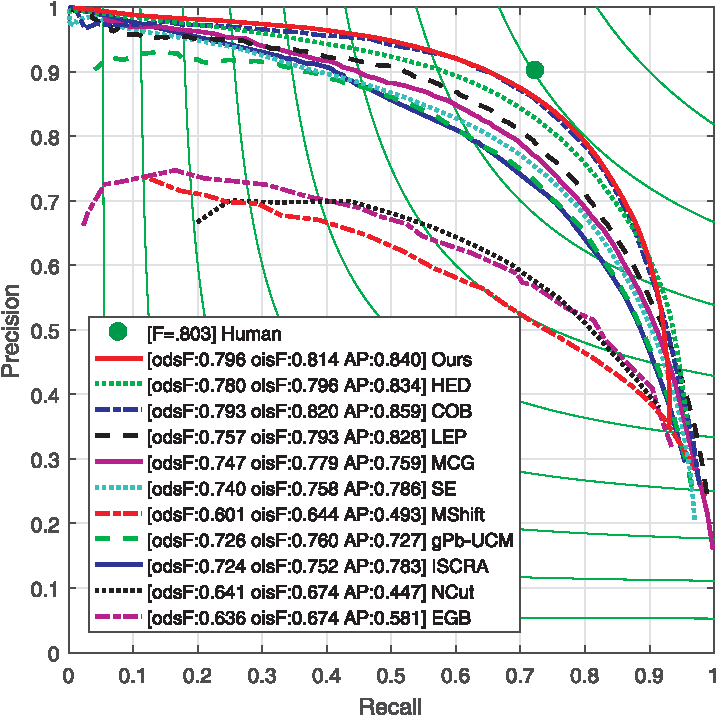
\includegraphics[width=0.98\linewidth]{boundary_prcurve}
   \vspace{-2mm}
   \caption{Boundary detection performance on BSDS500}
\label{fig:boundary_prcurve}
\vspace{-3mm}
\end{figure}

\begin{figure}[t]
\centering
   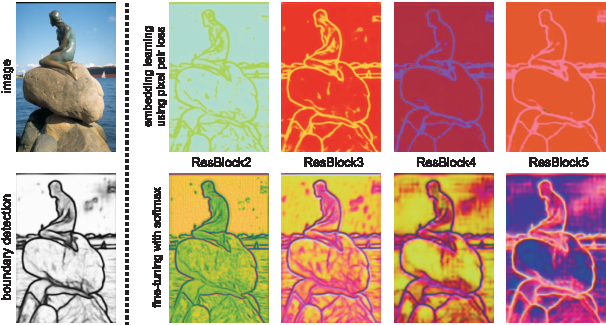
\includegraphics[width=1\linewidth]{boundary_show_in_paper_littleMermaid}
\vspace{-5mm}
   \caption{
   Visualization of boundary detection embeddings.  We show the 3D embedding as
   RGB images (more examples in appendix).  The upper and lower row in the
   right panel show embedding vectors at different layers from the model before
   and after fine-tuning using logistic loss.  After fine-tuning not only
   predict the boundary pixels, but also encode boundary orientation and signed
   distance to the boundary, similar to supervised embedding approaches
   \cite{sironi2014multiscale,uhrig2016pixel,bai2016deep}
   }
\label{fig:boundary_show_in_paper}
\vspace{-2mm}
\end{figure}


For boundary detection, we first train a model to group the pixels into
boundary or non-boundary groups.  Similar to
COB~\cite{maninis2017convolutional} and HED~\cite{xie2015holistically}, we
include multiple branches over ResBlock $2, 3, 4, 5$ for training.
Since the number of instances labels is 2, we learn a simple 3-dimensional
embedding space which has the advantage of easy visualization as an RGB
image.  Fig.~\ref{fig:boundary_show_in_paper} shows the resulting embeddings
in the first row of each panel.  Note that even though we didn't utilize
mean-shift grouping, the trained embedding already produces compact clusters.
To compare quantitatively to the state-of-the-art, we learn a fusion
layer that combines predictions from multiple levels of the feature
hierarchy fine-tuned with a logistic loss to match the binary output.
Fig.~\ref{fig:boundary_show_in_paper} shows the results in the second row.
Interestingly, we can see that the fine-tuned model embeddings
encode not only boundary presence/absence but also the orientation
and signed distance to nearby boundaries.

Quantitatively,
we compare our model to
COB~\cite{maninis2017convolutional},
HED~\cite{xie2015holistically},
CEDN~\cite{yang2016object},
LEP~\cite{najman1996geodesic},
UCM~\cite{arbelaez2011contour},
ISCRA~\cite{ren2013image},
NCuts~\cite{shi2000normalized},
EGB~\cite{felzenszwalb2004efficient},
and the original mean shift (MShift) segmentation algorithm~\cite{comaniciu2002mean}.
Fig.~\ref{fig:boundary_prcurve} shows standard benchmark precision-recall for
all the methods, demonstrating our model achieves state-of-the-art performance.
Note that our model has the same architecture of COB~\cite{maninis2017convolutional}
except with a different
loss functions and no explicit branches to compute boundary orientation.  Our
embedding loss by naturally pushes boundary pixel embeddings to be similar
which is also the desirable property for detecting boundaries using logistic
loss.  Note that it is possible to surpass human performance with several
sophisticated techniques~\cite{kokkinos2015pushing}, we don't pursue
this as it is out the scope of this paper.


\subsection{Object Proposal Detection}
\begin{figure}[t]
\centering
   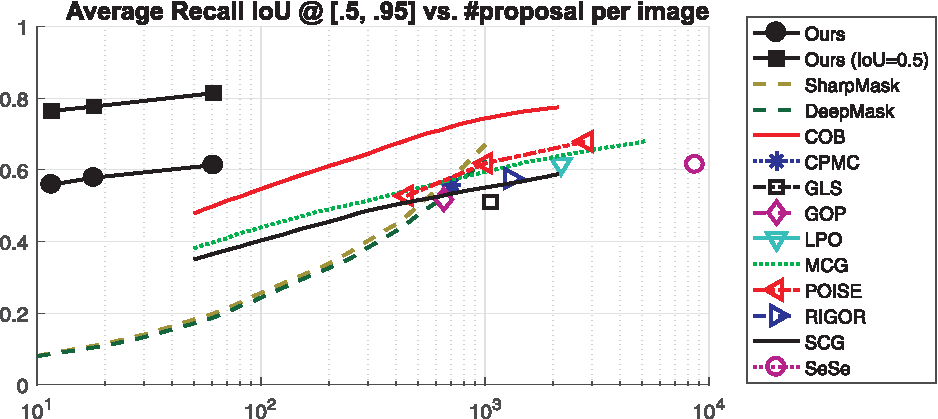
\includegraphics[width=1\linewidth]{plot_perf_objPropDet}
   \vspace{-6mm}
   \caption{Segmented object proposals evaluation on PASCAL VOC 2012 validation
   set measured by Average Recall (AR) at IoU from 0.5 to 0.95 and step size as 0.5.
   We also include the curve for our method at IoU=0.5.
   }
\label{fig:plot_perf_objPropDet}
%\vspace{-1mm}
\end{figure}

Object proposals are an integral part of current object detection and semantic
segmentation pipelines~\cite{ren2015faster, he2017mask}, as they provide a
reduced search space of locations, scales and shapes for subsequent
recognition.  State-of-the-art methods usually involve training models that
output large numbers of proposals, particularly those based on bounding boxes.
Here we demonstrate that by training our framework with 64-dimensional
embedding space on the object instance level annotations, we are able to
produce very high quality object proposals by grouping the pixels into
instances.  It is worth noting that due to the nature of our grouping module,
far fewer number of proposals are produced with much higher quality.  We
compare against the most recent techniques including
POISE~\cite{humayun2015middle},
LPO~\cite{krahenbuhl2015learning},
CPMC~\cite{carreira2012cpmc},
GOP~\cite{krahenbuhl2014geodesic},
SeSe~\cite{uijlings2013selective},
GLS~\cite{rantalankila2014generating},
RIGOR~\cite{humayun2014rigor}.

%Recent thorough comparisons can be found in~\cite{hosang2016makes}.
%We perform experiment on the PASCAL VOC 2012 dataset~\cite{everingham2010pascal} augmented by SDB dataset~\cite{hariharan2011semantic}.

Fig.~\ref{fig:plot_perf_objPropDet} shows the Average Recall
(AR)~\cite{hosang2016makes} with respect to the number of object
proposals\footnote{Our basic model produces $\sim10$ proposals per image.  In order
to plot a curve for our model for larger numbers of proposals, we run the mean
shift grouping with multiple smaller bandwidth parameters, pool the results,
and remove redundant proposals.}. Our model performs remarkably well compared
to other methods, achieving high average recall of ground-truth objects with two
orders of magnitude fewer proposals.  We also plot the curves for
SharpMask~\cite{pinheiro2015learning} and DeepMask~\cite{pinheiro2016learning}
using the proposals released by the authors. Despite only training on PASCAL,
we outperform these models which were trained on the much larger COCO dataset~\cite{lin2014microsoft}.
In Table~\ref{tab:objProposalDet} we report the total average recall at
IoU$=0.5$ for some recently proposed proposal detection methods, including
unpublished work inst-DML~\cite{fathi2017semantic} which is similar in spirit
to our model but learns a Euclidean distance based metric to group pixels.
We can clearly see that our method achieves significantly better results than
existing methods.

{
\setlength{\tabcolsep}{0.25em}
\begin{table}%[th]
\centering
{\footnotesize
\begin{tabular}{c | c c c  c |  c  }
\hline
 $\#$prop. & SCG~\cite{pont2017multiscale}
                     & MCG~\cite{pont2017multiscale}
                     & COB~\cite{maninis2017convolutional}
                     & inst-DML~\cite{fathi2017semantic}
                     & Ours      \\
\hline
10               & -            & -         & -     &  0.558     & 0.769 \\
60               & 0.624        & 0.652     & 0.738 &  0.667     & 0.814 \\
%150               & -        & -     & 81.6 &  -     & - \\
%500               & -        & 81.9     & - &  82.2     & - \\
%700               & 81.4        & -     & - &  -     & - \\
\hline
\end{tabular}
}
\vspace{-3mm}
\caption{Object proposal detection on PASCAL VOC 2012 validation set measured
by total Average Recall (AR) at IoU=0.50 and various number of proposals per image.}
\vspace{-2mm}
\label{tab:objProposalDet}
\end{table}
}



\begin{figure}[t]
\centering
   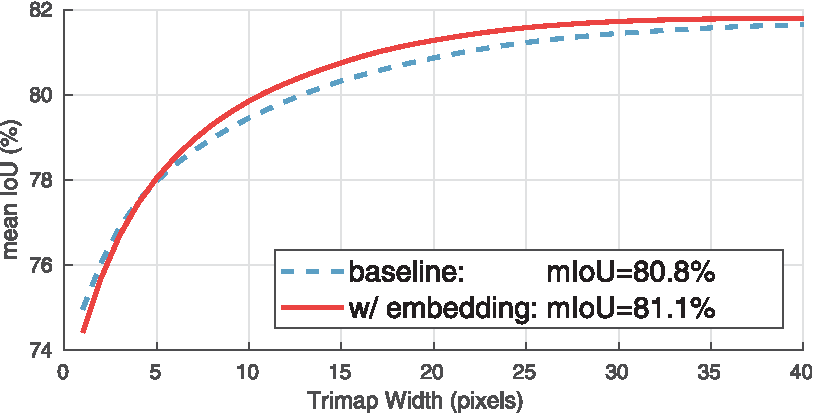
\includegraphics[width=0.80\linewidth]{trimap_semanticSeg_range40} % trimap_semanticSeg
   \vspace{-2mm}
   \caption{Semantic segmentation performance as a function of distance from ground-truth
   object boundaries comparing a baseline model trained with cross-entropy loss versus a
   model which also includes embedding loss.
   }
\label{fig:trimap_semanticSeg}
\vspace{-1mm}
\end{figure}

\begin{figure}[t]
\centering
   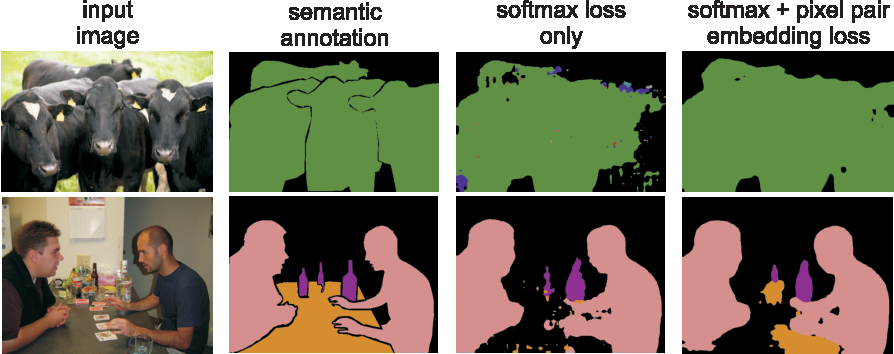
\includegraphics[width=1\linewidth]{semantic_seg_demo_2images} % semantic_seg_demo_3images
   \vspace{-5mm}
   \caption{The proposed embedding loss improves semantic segmentation by
   forcing the pixel feature vectors to be similar within the segments.
   Randomly selected images from PASCAL VOC2012 validation set.}
\label{fig:semantic_seg_demo}
\vspace{-3mm}
\end{figure}

\begin{figure*}[ht]
\centering
   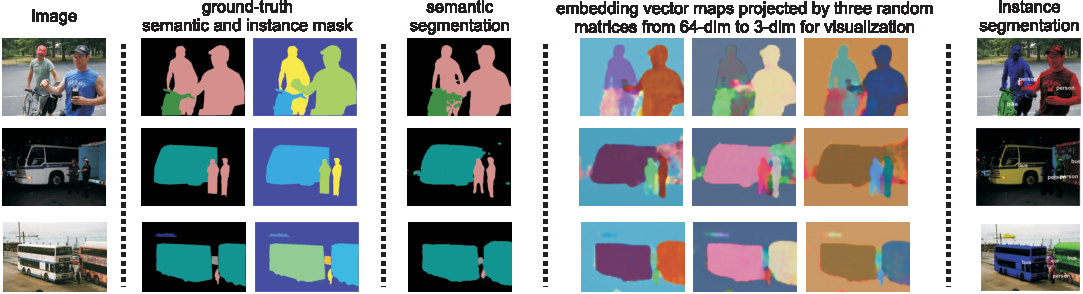
\includegraphics[width=0.99\linewidth]{instSeg_show_in_paper}
   \vspace{-3mm}
   \caption{Visualization of generic/instance-level semantic segmentation on
   random PASCAL VOC 2012 validation images.
   }
\label{fig:instSeg_show_in_paper}
\vspace{-1mm}
\end{figure*}


\begin{comment}
{
\setlength{\tabcolsep}{0.3em} % for the horizontal padding
\begin{table*}[!htbp]
\scriptsize
\begin{center}
\begin{tabular}{| c | c c c c c c c c c c c c c c c c c c c c | c |}
\hline
\scriptsize{Method} & \begin{sideways}\scriptsize{plane}\end{sideways} & \begin{sideways}\scriptsize{bike}\end{sideways} & \begin{sideways}\scriptsize{bird}\end{sideways} & \begin{sideways}\scriptsize{boat}\end{sideways} & \begin{sideways}\scriptsize{bottle}\end{sideways} & \begin{sideways}\scriptsize{bus}\end{sideways} & \begin{sideways}\scriptsize{car}\end{sideways} & \begin{sideways}\scriptsize{cat}\end{sideways} & \begin{sideways}\scriptsize{chair}\end{sideways} & \begin{sideways}\scriptsize{cow}\end{sideways} & \begin{sideways}\scriptsize{table}\end{sideways} & \begin{sideways}\scriptsize{dog}\end{sideways} & \begin{sideways}\scriptsize{horse}\end{sideways} & \begin{sideways}\scriptsize{motor}\end{sideways} & \begin{sideways}\scriptsize{person}\end{sideways} & \begin{sideways}\scriptsize{plant}\end{sideways} & \begin{sideways}\scriptsize{sheep}\end{sideways} & \begin{sideways}\scriptsize{sofa}\end{sideways} & \begin{sideways}\scriptsize{train}\end{sideways} & \begin{sideways}\scriptsize{tv}\end{sideways}  & \begin{sideways}\scriptsize{mean}\end{sideways} \\ \hline \hline
     SDS \cite{hariharan2014simultaneous}         & 58.8 & 0.5  & 60.1 & 34.4 & 29.5 & 60.6 & 40.0 & 73.6 & 6.5  & 52.4 & 31.7 & 62.0 & 49.1 & 45.6 & 47.9 & 22.6 & 43.5 & 26.9 & 66.2 & 66.1 & 43.8 \\
     Chen et al. \cite{chen2015multi} & 63.6 & 0.3  & 61.5 & 43.9 & 33.8 & 67.3 & 46.9 & 74.4 & 8.6  & 52.3 & 31.3 & 63.5 & 48.8 & 47.9 & 48.3 & 26.3 & 40.1 & 33.5 & 66.7 & 67.8 & 46.3 \\
     PFN \cite{liang2015proposal}     & 76.4 & 15.6 & 74.2 & 54.1 & 26.3 & 73.8 & 31.4 & 92.1 & 17.4 & 73.7 & 48.1 & 82.2 & 81.7 & 72.0 & 48.4 & 23.7 & 57.7 & 64.4 & 88.9 & 72.3 & 58.7 \\
     MNC \cite{dai2016instance}            & -    & -    & -    & -    & -    & -    & -    & -    & -    & -    & -    & -    & -    & -    & -    & -    & -    & -    & -    & -    & 63.5 \\
     Li et al. \cite{li2016fully}     & -    & -    & -    & -    & -    & -    & -    & -    & -    & -    & -    & -    & -    & -    & -    & -    & -    & -    & -    & -    & 65.7 \\
     R2-IOS \cite{liang2016reversible}          & 87.0 & 6.1  & 90.3 & 67.9 & 48.4 & 86.2 & 68.3 & 90.3 & 24.5 & 84.2 & 29.6 & 91.0 & 71.2 & 79.9 & 60.4 & 42.4 & 67.4 & 61.7 & 94.3 & 82.1 & 66.7 \\
     Assoc. Embed.~\cite{newell2016associative} & -    & -    & -    & -    & -    & -    & -    & -    & -    & -    & -    & -    & -    & -    & -    & -    & -    & -    & -    & -    & 35.1 \\
     inst-DML~\cite{fathi2017semantic}                             & 69.7    & 1.2    & 78.2    & 53.8    & 42.2    & 80.1    & 57.4    & 88.8    & 16.0    & 73.2    & 57.9    & 88.4    & 78.9    & 80.0    & 68.0    & 28.0    & 61.5    & 61.3    & 87.5    & 70.4    & 62.1    \\
     \hline
     Ours
        & 85.9 & 10.0 & 74.3 & 54.6 & 43.7
        & 81.3 & 64.1 & 86.1 & 17.5 & 77.5
        & 57.0 & 89.2 & 77.8 & 83.7 & 67.9
        & 31.2 & 62.5 & 63.3 & 88.6 & 74.2
     & 64.5   \\
    \hline
\end{tabular}
\vspace{-0.1in}
\end{center}
\caption{Instance-level segmentation comparison using APr metric at 0.5 IoU on the PASCAL VOC 2012 validation set.}
\vspace{-0.1in}
\label{tab:results_iou}
\end{table*}
}
\end{comment}


{
\setlength{\tabcolsep}{0.3em} % for the horizontal padding
\begin{table*}[!htbp]
\footnotesize
\begin{center}
\begin{tabular}{| c | c c c c c c c c c c c c c c c c c c c c | c |}
\hline
\footnotesize{Method} & \begin{sideways}\footnotesize{plane}\end{sideways} & \begin{sideways}\footnotesize{bike}\end{sideways} & \begin{sideways}\footnotesize{bird}\end{sideways} & \begin{sideways}\footnotesize{boat}\end{sideways} & \begin{sideways}\footnotesize{bottle}\end{sideways} & \begin{sideways}\footnotesize{bus}\end{sideways} & \begin{sideways}\footnotesize{car}\end{sideways} & \begin{sideways}\footnotesize{cat}\end{sideways} & \begin{sideways}\footnotesize{chair}\end{sideways} & \begin{sideways}\footnotesize{cow}\end{sideways} & \begin{sideways}\footnotesize{table}\end{sideways} & \begin{sideways}\footnotesize{dog}\end{sideways} & \begin{sideways}\footnotesize{horse}\end{sideways} & \begin{sideways}\footnotesize{motor}\end{sideways} & \begin{sideways}\footnotesize{person}\end{sideways} & \begin{sideways}\footnotesize{plant}\end{sideways} & \begin{sideways}\footnotesize{sheep}\end{sideways} & \begin{sideways}\footnotesize{sofa}\end{sideways} & \begin{sideways}\footnotesize{train}\end{sideways} & \begin{sideways}\footnotesize{tv}\end{sideways}  & \begin{sideways}\footnotesize{mean}\end{sideways} \\ \hline \hline
     SDS \cite{hariharan2014simultaneous}         & 58.8 & 0.5  & 60.1 & 34.4 & 29.5 & 60.6 & 40.0 & 73.6 & 6.5  & 52.4 & 31.7 & 62.0 & 49.1 & 45.6 & 47.9 & 22.6 & 43.5 & 26.9 & 66.2 & 66.1 & 43.8 \\
     Chen et al. \cite{chen2015multi} & 63.6 & 0.3  & 61.5 & 43.9 & 33.8 & 67.3 & 46.9 & 74.4 & 8.6  & 52.3 & 31.3 & 63.5 & 48.8 & 47.9 & 48.3 & 26.3 & 40.1 & 33.5 & 66.7 & 67.8 & 46.3 \\
     PFN \cite{liang2015proposal}     & 76.4 & 15.6 & 74.2 & 54.1 & 26.3 & 73.8 & 31.4 & 92.1 & 17.4 & 73.7 & 48.1 & 82.2 & 81.7 & 72.0 & 48.4 & 23.7 & 57.7 & 64.4 & 88.9 & 72.3 & 58.7 \\
     MNC \cite{dai2016instance}            & -    & -    & -    & -    & -    & -    & -    & -    & -    & -    & -    & -    & -    & -    & -    & -    & -    & -    & -    & -    & 63.5 \\
     Li et al. \cite{li2016fully}     & -    & -    & -    & -    & -    & -    & -    & -    & -    & -    & -    & -    & -    & -    & -    & -    & -    & -    & -    & -    & 65.7 \\
     R2-IOS \cite{liang2016reversible}          & 87.0 & 6.1  & 90.3 & 67.9 & 48.4 & 86.2 & 68.3 & 90.3 & 24.5 & 84.2 & 29.6 & 91.0 & 71.2 & 79.9 & 60.4 & 42.4 & 67.4 & 61.7 & 94.3 & 82.1 & 66.7 \\
     Assoc. Embed.~\cite{newell2016associative} & -    & -    & -    & -    & -    & -    & -    & -    & -    & -    & -    & -    & -    & -    & -    & -    & -    & -    & -    & -    & 35.1 \\
     inst-DML~\cite{fathi2017semantic}                             & 69.7    & 1.2    & 78.2    & 53.8    & 42.2    & 80.1    & 57.4    & 88.8    & 16.0    & 73.2    & 57.9    & 88.4    & 78.9    & 80.0    & 68.0    & 28.0    & 61.5    & 61.3    & 87.5    & 70.4    & 62.1    \\
     \hline
     Ours
        & 85.9 & 10.0 & 74.3 & 54.6 & 43.7
        & 81.3 & 64.1 & 86.1 & 17.5 & 77.5
        & 57.0 & 89.2 & 77.8 & 83.7 & 67.9
        & 31.2 & 62.5 & 63.3 & 88.6 & 74.2
     & 64.5   \\
    \hline

\end{tabular}
%\vspace{-0.1in}
\vspace{-5mm}
\end{center}
  \caption{Instance-level segmentation comparison using APr metric at 0.5 IoU on the PASCAL VOC 2012 validation set.}
\vspace{-2mm}
%\vspace{-0.1in}
\label{tab:results_iou}
\end{table*}
}


\subsection{Semantic Instance Detection}


As a final test of our method, we also train it to produce semantic labels
which are combined with our instance proposal method to recognize the detected
proposals.

For semantic segmentation which is a k-way classification problem, we train a
model using cross-entropy loss alongside our embedding loss.  Similar to our
proposal detection model, we use a 64-dimension embedding space on top of
DeepLab-v3~\cite{chen2017rethinking} as our base model.  While there are more
complex methods in literature such as PSPNet~\cite{zhao2016pyramid} and which
augment training with additional data (e.g., COCO~\cite{lin2014microsoft} or
JFT-300M dataset~\cite{sun2017revisiting}) and utilize ensembles and
post-processing, we focus on a simple experiment training the base model
with/without the proposed pixel pair embedding loss to demonstrate the
effectiveness. 

In addition to reporting mean intersection over union (mIoU) over all
classes,
%to better characterize performance differences between the two models,
we also computed mIoU restricted to a narrow band of pixels around the
ground-truth boundaries.  This partition into figure/boundary/background is
sometimes referred to as a tri-map in the matting literature and has been
previously utilized in analyzing semantic segmentation
performance~\cite{kohli2009robust, chen2016deeplab, ghiasi2016laplacian}.
Fig.~\ref{fig:trimap_semanticSeg} shows the mIoU as a function of the width
of the tri-map boundary zone.  This demonstrates that with embedding loss
yields performance gains over cross-entropy primarily far from ground-truth
boundaries where it successfully fills in holes in the segments output
(see also qualitative results in Fig.~\ref{fig:semantic_seg_demo}).
This is in spirit similar to the model in \cite{harley2017segmentation},
which considers local consistency to improve spatial precision.
However, our uniform sampling allows for long-range interactions between pixels.


To label detected instances with semantic labels, we use the semantic
segmentation model described above to generate labels and then use a simple
voting strategy to transfer these predictions to the instance proposals.  In
order to produce a final confidence score associated with each proposed object,
we train a linear regressor to score each object instance based on its
morphology (e.g., size, connectedness) and the consistency w.r.t. the semantic
segmentation prediction. We note this is substantially simpler than approaches
based, e.g. on Faster-RCNN~\cite{ren2015faster} which use much richer convolutional features to
rescore segmented instances~\cite{he2017mask}.

Comparison of instance detection performance are displayed in
Table~\ref{tab:results_iou}.  We use a standard IoU threshold of 0.5 to
identify true positives, unless an ground-truth instance has already been
detected by a higher scoring proposal in which case it is a false positive.  We
report the average precision per-class as well as the average all classes (as
in~\cite{hariharan2011semantic}).  Our approach yields competitive performance
on VOC validation despite our simple re-scoring.  Among the competing methods,
the one closest to our model is inst-DML~\cite{fathi2017semantic}, that learns
Euclidean distance based metric with logistic loss.  The inst-DML approach
relies on generating pixel seeds to derive instance masks.  The pixel seeds may
fail to correctly detect thin structures which perhaps explains why this method
performs 10x worse than our method on the bike category. In contrast, our
mean-shift grouping approach doesn't make strong assumptions about the
object shape or topology.

For visualization purposes, we generate three random matrices projections of
the 64-dimensional embedding and display them in the spatial domain as RGB
images.  Fig.~\ref{fig:instSeg_show_in_paper} shows the embedding
visualization, as well as predicted semantic segmentation and instance-level
segmentation.  From the visualization, we can see the instance-level semantic
segmentation outputs complete object instances even though semantic
segmentation results are noisy, such as the bike in the first image in
Fig.~\ref{fig:instSeg_show_in_paper}. The instance embedding provides
important details that resolve both inter- and intra-class instance overlap
which are not emphasized in the semantic segmentation loss.



